\subsection{Variational autoencoder}
\subsubsection{Problem scenario}
Assume that the data $\mathbb{X}=\left\lbrace x_i \right\rbrace^N_{i=1}$ are generated by some random process, involving and unobserved continuous variable $\boldsymbol{z}$, which will be referenced as a latent variable or code. The objective is once again to find the PDF of the given data in a parametric form $p_{\bt}\left(\bx\right)$. One can choose approximative distribution in the form of
\begin{equation}\label{eq:VAE_approxform}
p_{\bt}\left(\bx\right) = \int p_{\bt}\left(\bx,  \boldsymbol{z}\right)\d{\boldsymbol{z}} =\int p_{\bt}\left(\bx\vert \boldsymbol{z}\right)p_{\bt}\left(\boldsymbol{z}\right)\d{\boldsymbol{z}},
\end{equation}
but such approximation is usually very expensive to compute or can be even intractable. Intractability of the $p_{\bt}\left(\bx\right)$ makes posterior PDF $p_{\bt}\left(\boldsymbol{z}\vert\bx\right)$ also intractable.

\subsubsection{Naive approach}
One of the simplest ways to solve this problem may seem to be to build a model depending on the latent variable $f_{\bt}\left(\boldsymbol{z}\right)$ and try to train its parameters. For simplicity, let $p\left(\boldsymbol{z} \right) = \pazocal{N}\left(\boldsymbol{0}, \mathbb{I}_P\right)$, where $P$ denotes the dimension of the latent space $\boldsymbol{z}$ and also let
\begin{equation}
\bx = f_{\bt}\left(\boldsymbol{z}\right) + \boldsymbol{\varepsilon}, \quad \boldsymbol{\varepsilon} \sim \pazocal{N}\left(\boldsymbol{0},\sigma^2\cdot\mathbb{I}_D \right)
\end{equation}
which actually gives 
\begin{equation}\label{eq:VAE_decoder}
p_{\bt}\left(\bx\vert\boldsymbol{z}\right) = \pazocal{N}\left(\boldsymbol{x};f_{\bt}\left(\boldsymbol{z}\right),\sigma^2\cdot\mathbb{I}_D \right).
\end{equation}
The true PDF of the given data can be cleverly written using the empirical PDF, i.e. in the form of $p_{\mathrm{emp}}\left(\boldsymbol{x} \right)~=~\frac{1}{N}\sum_{i=1}^N\delta\left(\bx - \bx_i\right) $,
which can be exploited by finding the $\bt$ parameters by minimizing the $\KL{p_{\mathrm{emp}}\left(\boldsymbol{x} \right)}{p_{\bt}\left(\bx\right)}$. Since minimizing the KL distance is equivalent to ML estimation and using the approximative form \eqref{eq:VAE_approxform}, the following holds 
\begin{align}
    \widehat{\boldsymbol{\bt}} &= \argmin_{\boldsymbol{\bt}}- \sum_{i=1}^N\log p_{\boldsymbol{\bt}}\left(\boldsymbol{x}_i \right)\\
    &=  \argmin_{\boldsymbol{\bt}}- \sum_{i=1}^N \log \int \pazocal{N}\left(\boldsymbol{x}_i;f_{\bt}\left(\boldsymbol{z}\right),\sigma^2\cdot\mathbb{I}_D \right) \cdot \pazocal{N}\left(\boldsymbol{z};\boldsymbol{0}, \mathbb{I}_P\right) \d{\boldsymbol{z}}\\
    &= \argmin_{\boldsymbol{\bt}}- \sum_{i=1}^N \log \sum_{j=1}^{P}\exp\left(-\frac{1}{2\sigma^2}\left(\bx_i-f_{\bt}\left(\boldsymbol{z}_j\right)\right)^\top\left(\bx_i-f_{\bt}\left(\boldsymbol{z}_j\right)\right) \right).
\end{align}
Integration over $\boldsymbol{z}$ is represented by sampling. In iterations, for wrong value of $\bt$, all generated samples may
be away from samples of $\boldsymbol{x}$ and the gradient is poor.


\subsubsection{Variational Bayes approach}
\begin{figure}[h]
	\centering
	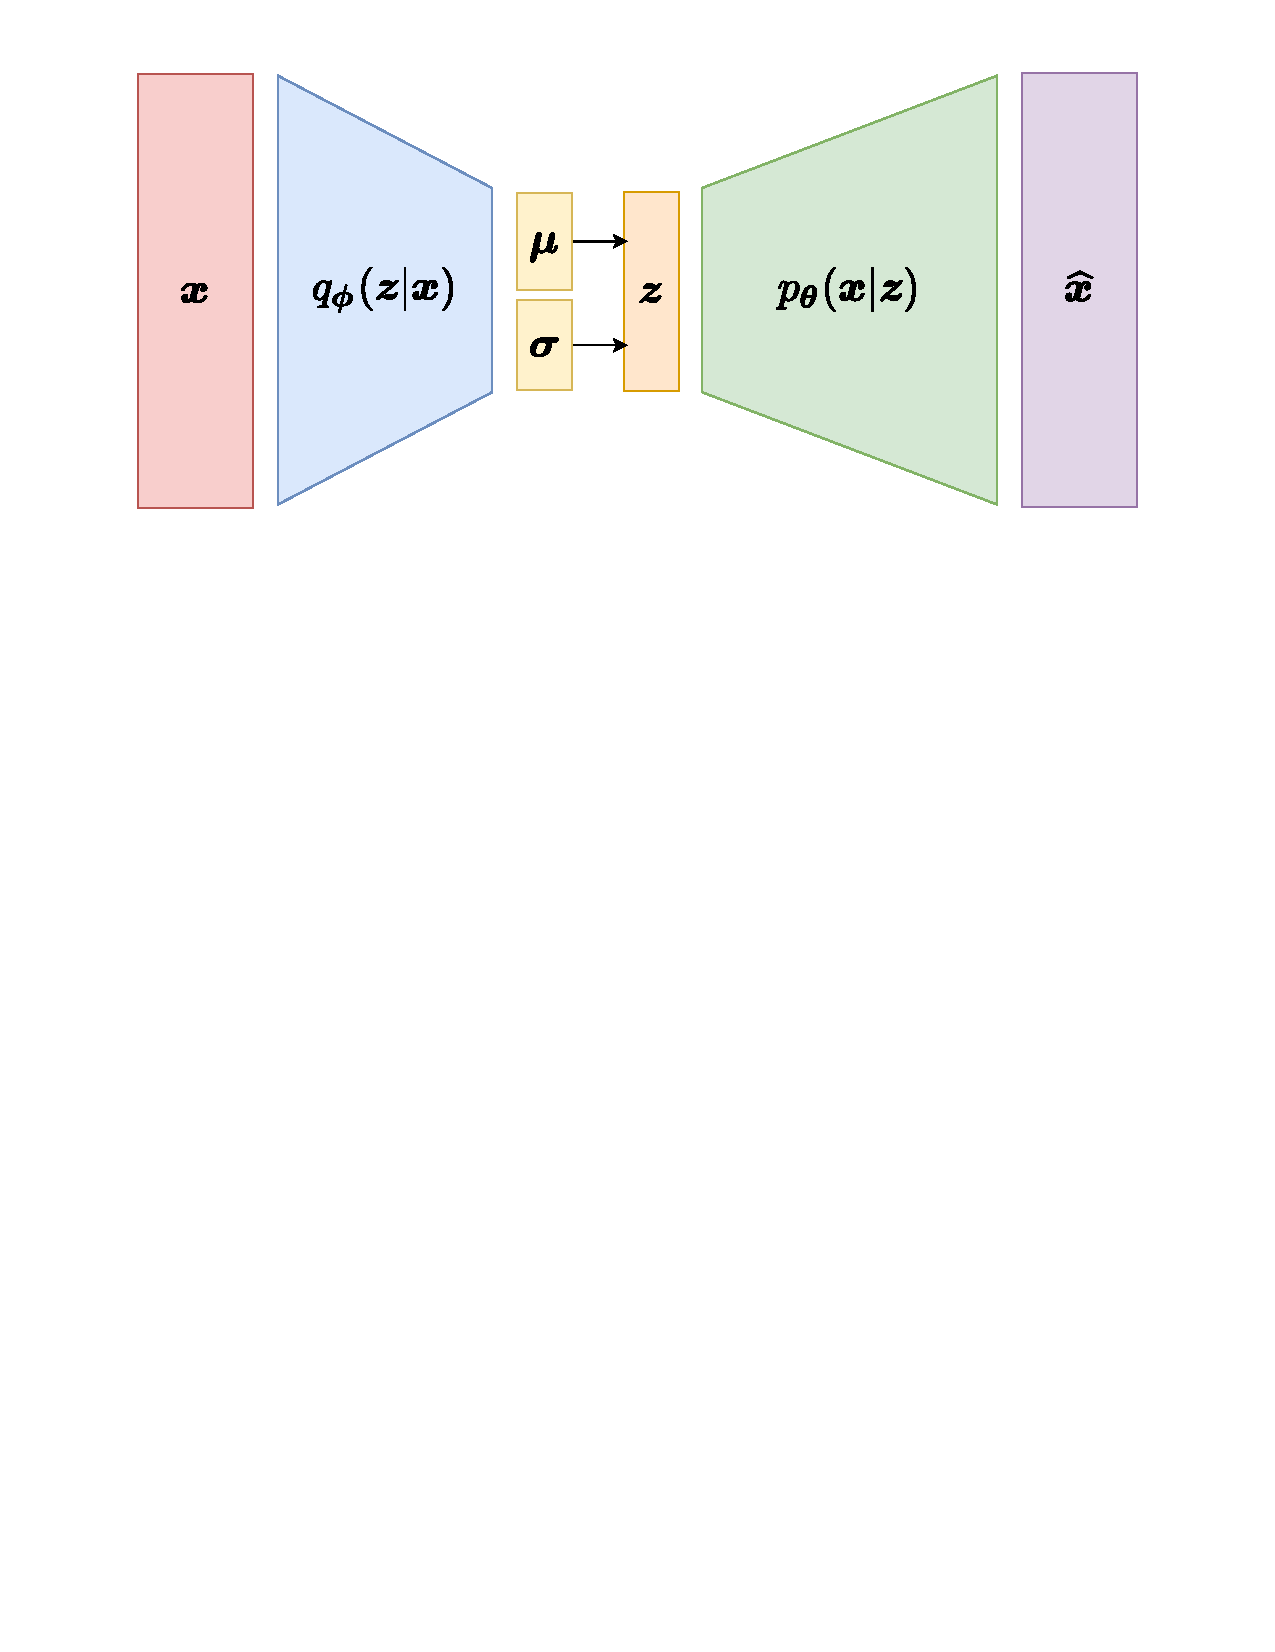
\includegraphics[width=\textwidth, trim={0 19cm 0 0cm}]{plots/Images/VAE_diagram.pdf}
	\caption{VAE diagram.}%
	\label{fig:VAE_architecture}%
\end{figure}

To solve this issue it is necessary to introduce further approximative posterior distribution $q_{\bphi}\left(\boldsymbol{z}\vert\bx\right) \approx p_{\bt}\left(\boldsymbol{z}\vert\bx\right)$ with parameters $\bphi$, preferably Gaussian. Standard terminology refers to the model $q_{\bphi}\left(\boldsymbol{z}\vert\bx\right)$ as a probabilistic \emph{encoder} and  $p_{\bt}\left(\bx\vert \boldsymbol{z}\right)$ is called a probabilistic \emph{decoder}. For variational autoencoder (VAE) the idea is to use KL distance from $q_{\bphi}\left(\boldsymbol{z}\vert\bx\right)$ to $p_{\bt}\left(\boldsymbol{z}\vert \bx\right)$, yielding
\begin{equation}\label{eq:VAEloss}
\begin{split}
D_{\mathrm{KL}}\left(q_{\bphi}\left(\boldsymbol{z}\vert \bx \right) \Vert p_{\bt}\left(\boldsymbol{z}\vert \bx\right)\right) & = 
\int q_{\bphi}\left(\boldsymbol{z}\vert \bx \right) \log \frac{q_{\bphi}\left(\boldsymbol{z}\vert \bx \right)}{p_{\bt}\left(\boldsymbol{z}\vert \bx\right)} \d{\boldsymbol{z}} \\
& =  \int q_{\bphi}\left(\boldsymbol{z}\vert \bx \right) \log \frac{q_{\bphi}\left(\boldsymbol{z}\vert \bx \right)p_{\bt}\left(\bx\right)}{p_{\bt}\left(\bx \vert \boldsymbol{z}\right) p_{\bt}\left(\boldsymbol{z}\right)} \d{\boldsymbol{z}} \\
& = \log p_{\bt}\left(\boldsymbol{x}\right) +  \int q_{\bphi}\left(\boldsymbol{z}\vert \bx \right) \log \frac{q_{\bphi}\left(\boldsymbol{z}\vert \bx \right)}{p_{\bt}\left(\bx \vert \boldsymbol{z}\right)p_{\bt}\left(\boldsymbol{z}\right) } \d{\boldsymbol{z}} \\
& = \log p_{\bt}\left(\boldsymbol{x}\right) +  \mathbb{E}_{q_{\bphi}\left(\boldsymbol{z}\vert \bx \right)}\left[\log\frac{q_{\bphi}\left(\boldsymbol{z}\vert \bx \right)}{p_{\bt}\left(\boldsymbol{z}\right)} - \log p\left(\textbf{x}\vert \boldsymbol{z}\right)\right]\\
    & = \log p_{\bt}\left(\boldsymbol{x}\right) +\KL{q_{\bphi}\left(\boldsymbol{z}\vert \bx \right)}{p_{\bt}\left(\boldsymbol{z}\right)} -  \mathbb{E}_{q_{\bphi}\left(\boldsymbol{z}\vert \bx \right)}\left[\log p\left(\bx\vert \boldsymbol{z}\right)\right].
 \end{split}
\end{equation}
Using the last equality of \eqref{eq:VAEloss}, it is possible to rewrite the equation into its typical form
\begin{equation}
\log p_{\bt}\left(\bx\right) - D_{\mathrm{KL}}\left(q_{\bphi}\left(\boldsymbol{z}\vert \bx \right) \Vert p_{\bt}(\boldsymbol{z}\vert \bx)\right) = \underbrace{\mathbb{E}_{q_{\bphi}\left(\boldsymbol{z}\vert \bx \right)}\left[\log p_{\bt}(\bx\vert \boldsymbol{z}) \right] - D_{\mathrm{KL}}\left(q_{\bphi}\left(\boldsymbol{z}\vert\bx \right) \Vert p_{\bt}\left(\boldsymbol{z}\right)\right)}_{\text{= $L\left(\bt,\bphi; \bx\right)$}},
\end{equation}
where the right hand side is called \emph{variational} lower bound. There is no uniformity in terminology and thus one can also encounter the name evidence lower bound (ELBO). The first term of the right hand side is known as reconstruction loss and the second term is often called regularization term. As a KL distance is always non-negative, it holds
\begin{equation}
    \log p_{\bt}\left(\bx\right) \geq L\left(\bt,\bphi; \bx\right).
\end{equation}
The objective is to maximize the log-likelihood $\log p_{\bt}\left(\bx\right)$ which is equivalent to minimizing the negative log-likelihood and that is what will be used here. At this point we have a lower bound for one datapoint $\bx$, but we need to include all observations in the lower bound. Joint log-likelihood can be rewritten as a sum over the marginal log-likelihoods of individual observations $\log p_{\bt}\left(\bx_1,\bx_2,\dots,\bx_N\right)~=~\sum_{i=1}^N\log p_{\bt}\left(\bx_i\right)$ which completes all the building blocks needed to determine the optimization equation. This formulation provides one major advantage, which is that it is now possible to jointly optimize both the generative parameters $\bt$ and the variational parameters $\bphi$ as follows 
\begin{align}
   \widehat{\bt}, \widehat{\bphi} &= \argmin_{\bt,\bphi}-\sum_{i=1}^N\log p_{\bt}\left(\bx_i\right)\\
   &=\argmin_{\bt,\bphi}-\sum_{i=1}^N L\left(\bt,\bphi; \bx_i\right)\\
  &= \argmin_{\bt,\bphi}-\sum_{i=1}^N\mathbb{E}_{q_{\bphi}\left(\boldsymbol{z}\vert \bx_i \right)}\left[\log p_{\bt}(\bx_i\vert \boldsymbol{z}) \right] - D_{\mathrm{KL}}\left(q_{\bphi}\left(\boldsymbol{z}\vert\bx_i \right) \Vert p_{\bt}\left(\boldsymbol{z}\right)\right).\label{eq:VAEloss}
\end{align}
For a better understanding of the problem, a diagram of the VAE is shown in the Figure \ref{fig:VAE_architecture}. Note that the latent space is usually much smaller than the input space and for this reason it is also sometimes called bottleneck. 


\subsubsection{Reparameterization trick}
\begin{wrapfigure}{r}{0.45\textwidth}
  \begin{center}
    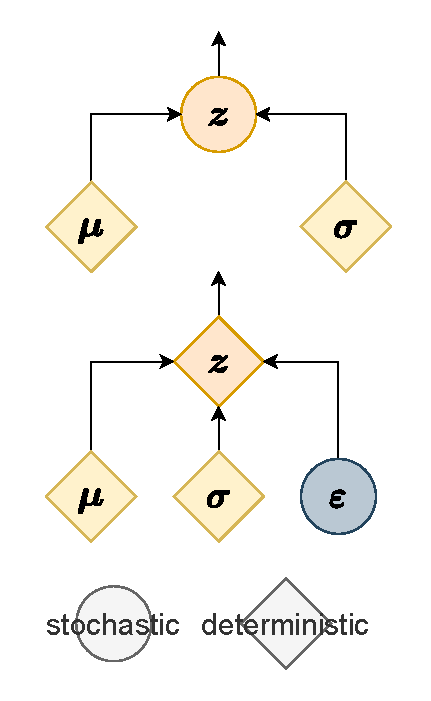
\includegraphics[trim={3cm 1.4cm 3cm 2.6cm}]{plots/Images/reparam_resized.pdf}
  \end{center}
  	\caption{Reparametrization trick.}%
	\label{fig:VAE_reparam}%
\end{wrapfigure}
The key success of VAE is in the fact that \eqref{eq:VAEloss} can be efficiently computed using the \emph{reparameterization trick}, where we express $\boldsymbol{z}$ as a deterministic variable
\begin{equation}\label{eq:reparam_general}
\boldsymbol{z} = g_{\bphi}\left(\boldsymbol{\varepsilon},\bx\right),
\end{equation}
 where $\boldsymbol{\varepsilon}$ stands for an auxiliary variable with independatnt marginal $p\left(\boldsymbol{\varepsilon}\right)$ and $g_{\bphi}\left(.\right)$ is a function parameterized by $\bphi$. 

A common explanation for this trick is that during the optimization the gradient cannot back--propagate through a random node. So, in the case of VAE, reparameterization trick shifts the source of randomness to another variable different than $\boldsymbol{z}$ and that allows differentiating with respect to $\boldsymbol{z}$. However, this explanation may not be sufficient and for this reason we will state a more formal justification. Consider taking the gradient with respect to $\bt$ of the $\mathbb{E}_{p(\bz)}\left[\model{z} \right]$. It can be easily computed as
\begin{align}
    \nabla_{\bt}  \mathbb{E}_{p(\bz)}\left[\model{z} \right] &= \nabla_{\bt} \int p(\bz) \model{z} \d{\bz} \\
    &= \int p(\bz) \nabla_{\bt} \model{z} \d{\bz} \\
    &=  \mathbb{E}_{p(\bz)}\left[\nabla_{\bt}\model{z} \right].\label{eq:nonparametricexpectation}
\end{align}
The result is obvious, the gradient of the expectation is equal to the expectation of the gradient. However, the gradient of the expectation becomes much more interesting if the PDF $p_{\bt}(\bz)$ is also parameterized by $\bt$, yielding
\begin{align}
    \nabla_{\bt}  \mathbb{E}_{p_{\bt}(\bz)}\left[\model{z} \right] &= \nabla_{\bt} \int p_{\bt}(\bz) \model{z} \d{\bz} \\
    &= \int p_{\bt}(\bz) \nabla_{\bt} \model{z} \d{\bz} + \int  \model{z} \nabla_{\bt}p_{\bt}(\bz)\d{\bz} \\
    &=  \mathbb{E}_{p_{\bt}(\bz)}\left[\nabla_{\bt}\model{z} \right] + \int  \model{z} \nabla_{\bt}p_{\bt}(\bz)\d{\bz}. \label{eq:paramexpectation}
\end{align}
The second term of \eqref{eq:paramexpectation} is not guaranteed to be an expectation and this very fact indicates that back--propagation would not compute an estimate of the $\nabla_{\bt}  \mathbb{E}_{p_{\bt}(\bz)}\left[\model{z} \right]$. In other words...(MonteCarlo). That being the case, if we apply the reparameterization trick $\bz =g_{\bt}\left(\boldsymbol{\varepsilon},\bx\right)$ to this simple example, we get
\begin{equation}
\mathbb{E}_{p_{\bt}(\bz)}\left[\model{z} \right] = \mathbb{E}_{p(\boldsymbol{\varepsilon})}\left[f\left(g_{\bt}(\boldsymbol{\varepsilon}, \bx)\right) \right].
\end{equation}
At this point, it is possible to take the gradient $\nabla_{\bt} \mathbb{E}_{p(\boldsymbol{\varepsilon})}\left[f\left(g_{\bt}(\boldsymbol{\varepsilon}, \bx)\right) \right]$ analogically as was done in \eqref{eq:nonparametricexpectation}. To be perfectly clear, authors of [] proposed an easy example: take the univariate Gaussian case $p(z|x) = \pazocal{N}\left(\mu, \sigma^2\right)$. In such a case, a proper reparametrization takes shape of
\begin{equation}\label{eq:VAE_reparam1D}
z = \mu + \sigma\varepsilon,
\end{equation}
where $\varepsilon\sim\pazocal{N}\left(0,1\right)$ and therefore the expectation
\begin{equation}
    \mathbb{E}_{\pazocal{N}\left(z;\mu, \sigma^2\right)}\left[f(z)\right] = \mathbb{E}_{\pazocal{N}\left(\varepsilon;0, 1\right)}\left[f(\mu + \sigma\varepsilon)\right] \approx \frac{1}{M}\sum_{j=1}^M f\left(\mu + \sigma\varepsilon_j\right).
\end{equation}
Note that this is nothing more than a transformation of a random variable. And this is exactly the issue with optimizing the ELBO \eqref{eq:VAEloss}. We need to rewrite the expectation $\mathbb{E}_{q_{\bphi}\left(\boldsymbol{z}\vert\bx_i \right)}$ so that the Monte Carlo estimate of the expected value is differentiable with respect to $\boldsymbol{\phi}$.

\subsubsection{Variational autoencoder}
So far we have only dealt with VAE in general. In this section we put everything together and specify the individual parts of the ELBO \eqref{eq:VAEloss}.
Let the probabilistic encoder be a multivariate Gaussian with a diagonal covariance matrix
\begin{equation}\label{eq:VAE_q}
q_{\bphi}\left(\boldsymbol{z}\vert \bx \right) = \pazocal{N}\left(\boldsymbol{z}; \boldsymbol{\mu},\boldsymbol{\sigma}^2\mathbb{I}_P  \right) 
\end{equation}
and let the probabilistic decoder takes the form depending on the type of given data and model. Finally, let the prior $p_{\bt}\left(\bz\right)$ be the centered izotropic multivariate Gaussian, i.e.
\begin{equation}
p_{\bt}\left(\boldsymbol{z} \right) = p\left(\boldsymbol{z} \right) = \pazocal{N}\left(\boldsymbol{z}; \boldsymbol{0},\mathbb{I}_P  \right),
\end{equation}
where generative parameters $\bt$ are omitted, since the chosen prior lacks parameters. When using \eqref{eq:VAE_q}, $\boldsymbol{\mu}$ and $\boldsymbol{\sigma}$ are non--linear functions of datapoint $\bx$ and variational parameters $\bphi$. This setting actually allows to take the reparametrization trick in a similar form as in \eqref{eq:VAE_reparam1D}, that means
\begin{equation}\label{eq:reparam_specific}
\boldsymbol{z}_{i,j} = \boldsymbol{\mu}_i + \boldsymbol{\sigma}_i\odot\boldsymbol{\varepsilon}_j ,
\end{equation}
where the symbol $\odot$ denotes Hadamard product, i.e. element-wise product and $\boldsymbol{\varepsilon} \sim \pazocal{N}\left(\boldsymbol{0},\mathbb{I} \right)$.
Another important fact is that the KL distance from a Gaussian distribution to a Gaussian distribution has an analytical solution, so $\KL{q_{\bphi}\left(\bz\vert \bx \right)}{p_{\bt}\left(\bz\right)}$ can be expressed in closed form:
\begin{equation}
\begin{split}
 \KL{q_{\bphi}\left(\bz\vert \bx \right)}{p_{\bt}\left(\bz\right)} & = \KL{\pazocal{N}\left(\boldsymbol{z}; \boldsymbol{\mu},\boldsymbol{\sigma}^2\mathbb{I}_P  \right) }{\pazocal{N}\left(\boldsymbol{z}; \boldsymbol{0},\mathbb{I}_P  \right)}\\ & =\frac{1}{2}\sum_{j=1}^P\left(1 + \log\sigma^2_j -\mu_j^2 -\sigma_j^2 \right).
\end{split}
\end{equation}
Now all that is left is to plug everything into the equation \eqref{eq:VAEloss} which leads to the final form
\begin{align}\label{řešení_VAE}
 \widehat{\bt}, \widehat{\bphi} & = \argmin_{\bt,\bphi}-\sum_{i=1}^N\mathbb{E}_{q_{\bphi}\left(\boldsymbol{z}\vert \bx_i \right)}\left[\log p_{\bt}(\bx_i\vert \boldsymbol{z}) \right] - D_{\mathrm{KL}}\left(q_{\bphi}\left(\boldsymbol{z}\vert\bx_i \right) \Vert p_{\bt}\left(\boldsymbol{z}\right)\right) \\
 & = \argmin_{\bt, \bphi}-\sum_{i = 1}^N\sum_{j = 1}^P \left( \bx_i - f_{\bt}\left(\boldsymbol{\mu}_i + \boldsymbol{\sigma}_i\odot\boldsymbol{\varepsilon_{j}} \right)\right) ^2 -   \frac{1}{2}\sum_{j=1}^P\left(1 + \log\sigma^2_{i,j} -\mu_{i,j}^2 -\sigma_{i,j}^2 \right).
\end{align}

